\lecture{6}{How Expressive are Graph Neural Networks?}{Thursday, October 8, 2026}\label{ch:lec06}

% Local TikZ styles (prefix lec06)
\tikzset{
  lec06n/.style={circle, draw=black!55, fill=YellowOrange!70, minimum size=3.4mm,
                 inner sep=0pt, font=\scriptsize\sffamily},
  lec06rt/.style={lec06n, draw=black, very thick},
  lec06agg/.style={fill=ForestGreen!85!black, minimum width=3.4mm,
                   minimum height=1.1mm, inner sep=0pt},
  lec06up/.style={black!80, semithick, -{Stealth[length=1.2mm]}},
  lec06emb/.style={circle, minimum size=2.4mm, inner sep=0pt},
  lec06Y/.style={circle, fill=YellowOrange!80, minimum size=3.2mm, inner sep=0pt},
  lec06B/.style={circle, fill=SkyBlue!90!black, minimum size=3.2mm, inner sep=0pt},
  lec06G/.style={circle, fill=ForestGreen!60, minimum size=3.2mm, inner sep=0pt},
  lec06R/.style={circle, fill=WildStrawberry!60, minimum size=3.2mm, inner sep=0pt},
  lec06ctr/.style={circle, fill=BurntOrange!85, text=white, minimum size=4.2mm,
                   inner sep=0pt, font=\scriptsize\sffamily\bfseries},
  lec06ms/.style={draw, thick, rounded corners=2pt},
  lec06vec/.style={font=\scriptsize, inner sep=1pt},
  lec06lbl/.style={font=\scriptsize\sffamily},
  lec06both/.style={black!50, line width=1.3pt,
                    {Stealth[length=2mm]}-{Stealth[length=2mm]}},
  lec06wl/.style={ellipse, draw=black!70, fill=black!8, inner sep=0.4pt,
                  minimum height=3.3mm, minimum width=4.2mm, font=\tiny\sffamily},
  lec06s/.style={circle, fill=blue!14, minimum size=3.4mm, inner sep=0pt,
                 font=\tiny\itshape},
  % the two graphs of the color-refinement example (slides 51--53)
  pics/lec06wlL/.style n args={6}{code={
    \node[lec06wl] (-tl) at (-0.5,0.62) {#1};
    \node[lec06wl] (-tr) at (0.5,0.62) {#2};
    \node[lec06wl] (-l)  at (-1.0,0) {#3};
    \node[lec06wl] (-r)  at (1.0,0) {#4};
    \node[lec06wl] (-bl) at (-0.5,-0.62) {#5};
    \node[lec06wl] (-br) at (0.5,-0.62) {#6};
    \draw[black!70] (-tl)--(-tr) (-tl)--(-l) (-tl)--(-r) (-tr)--(-r)
      (-l)--(-r) (-l)--(-bl) (-l)--(-br);
  }},
  pics/lec06wlR/.style n args={6}{code={
    \node[lec06wl] (-tl) at (-0.5,0.62) {#1};
    \node[lec06wl] (-tr) at (0.5,0.62) {#2};
    \node[lec06wl] (-l)  at (-1.0,0) {#3};
    \node[lec06wl] (-r)  at (1.0,0) {#4};
    \node[lec06wl] (-bl) at (-0.5,-0.62) {#5};
    \node[lec06wl] (-br) at (0.5,-0.62) {#6};
    \draw[black!70] (-tl)--(-tr) (-tl)--(-l) (-l)--(-tr) (-tr)--(-r)
      (-l)--(-r) (-l)--(-bl) (-r)--(-br);
  }},
}

\textbf{Outline.} Recap $\to$ local neighborhood structures and computational
graphs (rooted subtrees) $\to$ injective neighbor aggregation $\to$ failure cases
of GCN (mean-pool) and GraphSAGE (max-pool) $\to$ injective multi-set functions
and GIN $\to$ WL graph kernel and the complete GIN model $\to$ limits of WL/GIN
and improvements.

% ---------------------------------------------------------------------
\section{How expressive are GNNs?}\label{sec:lec06-expressive}

\subsection{Recap and motivation}\label{sec:lec06-recap}
\slides{3--6}

\begin{itemize}
  \item \textbf{Recap -- GNN training pipeline} (\cref{ch:lec05}): input graph
    $\to$ graph neural network $\to$ node embeddings $\to$ \textbf{prediction
    head} $\to$ predictions; predictions vs.\ \textbf{labels} $\to$ \textbf{loss
    function}, \textbf{evaluation metrics}; plus \textbf{dataset split}.
    Implementation resources: \textbf{PyG} provides core modules for this
    pipeline; \textbf{GraphGym} further implements the full pipeline to
    facilitate GNN design.
  \item \textbf{Information modalities in graphs:} social networks, economic
    networks, citation networks, molecules.
  \item \textbf{Why is graph deep learning hard? Graphs are complex:} complex
    topological structure (i.e.\ no spatial locality like grids; networks vs.\
    images, text); no fixed node ordering or reference point.
  \item \textbf{Theory of GNNs -- how powerful are GNNs?}
    \begin{itemize}
      \item Many GNN models have been proposed (e.g.\ GCN, GAT, GraphSAGE, design
        space).
      \item What is the \term{expressive power} (ability to distinguish
        different graph structures) of these GNN models?
      \item How to design a \textbf{maximally expressive} GNN model?
    \end{itemize}
\end{itemize}

\subsection{Graph isomorphism and a simpler problem}\label{sec:lec06-iso}
\slides{7--8}

\begin{itemize}
  \item \textbf{A classical expressivity test is \term{graph isomorphism}:} given a
    pair of graphs, can we tell if they are isomorphic? (Slide pair: the 5-node
    graph of \cref{fig:lec06-subtrees}, edges 1--2, 1--5, 2--5, 4--5, 3--4, vs.\
    the same graph plus edge 2--4.)
  \item \textbf{Open problem} (a polynomial time algorithm does not exist, has
    not been proven NP-complete).
  \item \textbf{A simpler problem:} given a pair of nodes with different
    neighborhood structures, is there a GNN that can always tell them apart?
    (Slide shows the graph and every node's computational graph,
    \cref{fig:lec06-subtrees}.)
\end{itemize}
\begin{caution}
  Slides~7, 49 say a polynomial-time algorithm ``does not exist''; correct: none
  is \emph{known}.
\end{caution}

\subsection{Background: message-passing GNNs}\label{sec:lec06-background}
\slides{9--12}

We focus on \textbf{message passing GNNs} (\cref{ch:lec04}): (1)
\textbf{Message:} each node computes a message; (2) \textbf{Aggregation:}
aggregate messages from neighbors:
\begin{equation}\label{eq:lec06-msgagg}
  \vm_u^{(l)} = \MSG^{(l)}\big(\vh_u^{(l-1)}\big),\ u\in\{N(v)\cup v\};
  \qquad
  \vh_v^{(l)} = \AGG^{(l)}\big(\{\vm_u^{(l)}, u\in N(v)\},\,\vm_v^{(l)}\big)
\end{equation}
\begin{itemize}
  \item Many GNN models have been proposed: GCN, GraphSAGE, GAT, Design Space
    etc. On the computational graph of a target node ($A$, neighbors $B,C,D$, in
    the $A$--$F$ input graph), \textbf{different GNN models use different neural
    networks in the box}:
    \begin{itemize}
      \item \textbf{GCN (mean-pool)} [Kipf and Welling ICLR 2017]: element-wise
        mean pooling + Linear + ReLU non-linearity.
      \item \textbf{GraphSAGE (max-pool)} [Hamilton et al.\ NeurIPS 2017]: MLP +
        element-wise max-pooling.
    \end{itemize}
\end{itemize}

\subsection{Local neighborhood structures}\label{sec:lec06-local}
\slides{13--17}

\begin{itemize}
  \item \textbf{Node colors:} same/different \textbf{colors} represent nodes with
    same/different features; e.g.\ the graph of \cref{fig:lec06-subtrees} assumes
    all the nodes share the same feature.
  \item \textbf{Key question:} how well can a GNN distinguish different graph
    structures?
  \item We specifically consider \term{local neighborhood structures} around each
    node in a graph:
    \begin{itemize}
      \item Nodes 1 and 5: \textbf{different} neighborhood structures because they
        have different node degrees.
      \item Nodes 1 and 4: both degree 2, but still \textbf{different}, because
        \textbf{their neighbors have different node degrees} (node 1: neighbors of
        degrees 2 and 3; node 4: neighbors of degrees 1 and 3).
      \item Nodes 1 and 2: the \textbf{same} neighborhood structure because
        \textbf{they are symmetric within the graph} (both: neighbors of degrees 2
        and 3; even a step deeper, 2nd-hop neighbors have the same degrees (node 4
        of degree 2)).
    \end{itemize}
  \item \textbf{Key question:} can GNN node embeddings distinguish different
    node's local neighborhood structures? If so, when? If not, when will a GNN
    fail?
  \item \textbf{Next:} understand how a GNN captures local neighborhood
    structures. Key concept: \term{computational graph}.
\end{itemize}

\subsection{Computational graphs = rooted subtrees}\label{sec:lec06-compgraph}
\slides{18--24}

\begin{itemize}
  \item \textbf{In each layer, a GNN aggregates neighboring node embeddings.} A
    GNN generates node embeddings through a \textbf{computational graph defined by
    the neighborhood}. Ex.: node 1's computational graph (2-layer GNN):
    $1\leftarrow\{2,5\}$, $2\leftarrow\{1,5\}$, $5\leftarrow\{1,2,4\}$.
  \item Nodes 1 and 2's computational graphs: node 2: $2\leftarrow\{1,5\}$,
    $1\leftarrow\{2,5\}$, $5\leftarrow\{1,2,4\}$. \textbf{But GNN only sees node
    features (not IDs)} $\Rightarrow$ the two trees look identical.
  \item \textbf{A GNN will generate the same embedding for nodes 1 and 2}
    because: computational graphs are the same; node features (colors) are
    identical. (GNN does not care about node ids, it just aggregates feature
    vectors of different nodes.) $\Rightarrow$ \textbf{GNN won't be able to
    distinguish nodes 1 and 2. (this is assuming that the features of all the embeddings are the same)}
  \item In general, \textbf{different local neighborhoods define different
    computational graphs} (\cref{fig:lec06-subtrees}).
  \item Computational graphs are identical to \term{rooted subtree structures}
    around each node (defined by recursively unfolding neighboring nodes from the
    root nodes).
  \item \textbf{GNN's node embeddings capture rooted subtree structures.} The
    \textbf{most expressive GNN} maps different rooted subtrees into different node
    embeddings (represented by different colors; top row of
    \cref{fig:lec06-subtrees}).
\end{itemize}

\begin{figure}[htbp]
  \centering
  \begin{tikzpicture}
    % input graph
    \node[lec06rt] (g1) at (0,-0.35) {1};
    \node[lec06rt] (g2) at (1.3,-0.35) {2};
    \node[lec06n]  (g3) at (2.0,-0.85) {3};
    \node[lec06n]  (g5) at (0,-1.45) {5};
    \node[lec06n]  (g4) at (1.3,-1.45) {4};
    \draw[edge] (g1)--(g2) (g1)--(g5) (g2)--(g5) (g5)--(g4) (g4)--(g3);
    \node[lec06lbl] at (1.0,-2.0) {input graph};
    % embedding row (slide 24)
    \draw[thick, rounded corners=2pt] (2.75,0.32) rectangle (12.75,0.78);
    \node[lec06lbl, anchor=south east, text=ForestGreen!70!black] at (12.75,0.78) {embedding};
    \foreach \x/\c in {3.735/Salmon, 5.985/Salmon, 7.71/TealBlue, 8.92/Green, 11.40/Plum}
      \node[lec06emb, fill=\c] at (\x,0.55) {};
    % tree of node 1
    \node[lec06rt] (r) at (3.735,0) {1};
    \node[lec06agg] (rb) at (3.735,-0.45) {}; \draw[lec06up] (rb)--(r);
    \foreach \n/\x/\c in {2/3.21/a, 5/4.26/b} {
      \node[lec06n] (k\c) at (\x,-0.9) {\n};
      \node[lec06agg] (q\c) at (\x,-1.35) {};
      \draw[lec06up] (q\c)--(k\c); \draw[lec06up] (k\c)--(rb);}
    \foreach \n/\x/\c in {1/3.0/a, 5/3.42/a, 1/3.84/b, 2/4.26/b, 4/4.68/b} {
      \node[lec06n] (lf) at (\x,-1.8) {\n}; \draw[lec06up] (lf)--(q\c);}
    % tree of node 2
    \node[lec06rt] (r) at (5.985,0) {2};
    \node[lec06agg] (rb) at (5.985,-0.45) {}; \draw[lec06up] (rb)--(r);
    \foreach \n/\x/\c in {1/5.46/a, 5/6.51/b} {
      \node[lec06n] (k\c) at (\x,-0.9) {\n};
      \node[lec06agg] (q\c) at (\x,-1.35) {};
      \draw[lec06up] (q\c)--(k\c); \draw[lec06up] (k\c)--(rb);}
    \foreach \n/\x/\c in {2/5.25/a, 5/5.67/a, 1/6.09/b, 2/6.51/b, 4/6.93/b} {
      \node[lec06n] (lf) at (\x,-1.8) {\n}; \draw[lec06up] (lf)--(q\c);}
    % tree of node 3
    \node[lec06n] (r) at (7.71,0) {3};
    \node[lec06agg] (rb) at (7.71,-0.45) {}; \draw[lec06up] (rb)--(r);
    \node[lec06n] (ka) at (7.71,-0.9) {4};
    \node[lec06agg] (qa) at (7.71,-1.35) {};
    \draw[lec06up] (qa)--(ka); \draw[lec06up] (ka)--(rb);
    \foreach \n/\x in {3/7.5, 5/7.92} {
      \node[lec06n] (lf) at (\x,-1.8) {\n}; \draw[lec06up] (lf)--(qa);}
    % tree of node 4
    \node[lec06n] (r) at (8.92,0) {4};
    \node[lec06agg] (rb) at (8.92,-0.45) {}; \draw[lec06up] (rb)--(r);
    \foreach \n/\x/\c in {3/8.5/a, 5/9.34/b} {
      \node[lec06n] (k\c) at (\x,-0.9) {\n};
      \node[lec06agg] (q\c) at (\x,-1.35) {};
      \draw[lec06up] (q\c)--(k\c); \draw[lec06up] (k\c)--(rb);}
    \foreach \n/\x/\c in {4/8.5/a, 1/8.92/b, 2/9.34/b, 4/9.76/b} {
      \node[lec06n] (lf) at (\x,-1.8) {\n}; \draw[lec06up] (lf)--(q\c);}
    % tree of node 5
    \node[lec06n] (r) at (11.40,0) {5};
    \node[lec06agg] (rb) at (11.40,-0.45) {}; \draw[lec06up] (rb)--(r);
    \foreach \n/\x/\c in {1/10.56/a, 2/11.40/b, 4/12.24/c} {
      \node[lec06n] (k\c) at (\x,-0.9) {\n};
      \node[lec06agg] (q\c) at (\x,-1.35) {};
      \draw[lec06up] (q\c)--(k\c); \draw[lec06up] (k\c)--(rb);}
    \foreach \n/\x/\c in {2/10.35/a, 5/10.77/a, 1/11.19/b, 5/11.61/b, 3/12.03/c, 5/12.45/c} {
      \node[lec06n] (lf) at (\x,-1.8) {\n}; \draw[lec06up] (lf)--(q\c);}
  \end{tikzpicture}
  \caption{Input graph (all nodes share the same feature) and the 2-layer
  computational graphs = rooted subtrees of nodes 1--5 (green bars: aggregation).
  Nodes 1 and 2 have identical subtrees $\Rightarrow$ same embedding; top row: one
  embedding color per distinct subtree (slides~8, 18--24).}
  \label{fig:lec06-subtrees}
\end{figure}

\begin{caution}
  Slides~24, 26 draw node 3's subtree with the single leaf 5; correct (slides~8,
  22--23): leaves 3 and 5 (the neighbors of node 4).
\end{caution}

\subsection{Injective neighbor aggregation}\label{sec:lec06-injective}
\slides{25--30}

\begin{definition}[Injective function]\label{def:lec06-injective}
  Function $f: X\to Y$ is \term{injective} if it maps different elements into
  different outputs. \textbf{Intuition:} $f$ retains all the information about
  the input. (Slide example: $1\mapsto D$, $2\mapsto B$, $3\mapsto A$; $C$ not
  hit.)
\end{definition}
\begin{itemize}
  \item Most expressive GNN should map subtrees to the node embeddings
    \textbf{injectively} (subtrees $\to$ embedding space $\R^d$; the identical
    subtrees of nodes 1 and 2 map to the same point).
  \item \textbf{Key observation:} subtrees of the same depth can be
    \textbf{recursively characterized from the leaf nodes to the root nodes}. Ex.\
    (input features are uniform): node 1 = (2 neighbors, 3 neighbors)
    $\neq$ node 4 = (1 neighbor, 3 neighbors).
  \item If each step of GNN's aggregation can \textbf{fully retain the
    neighboring information}, the generated node embeddings can distinguish
    different rooted subtrees.
  \item In other words, most expressive GNN would use an \term{injective neighbor
    aggregation} function at each step: maps different neighbors to different
    embeddings.
\end{itemize}
\begin{keyidea}[Summary so far]
  To generate a node embedding, GNNs use a computational graph corresponding to a
  subtree rooted around each node (computational graph = rooted subtree). GNN can
  fully distinguish different subtree structures if \textbf{every step of its
  neighbor aggregation is injective}.
\end{keyidea}

% ---------------------------------------------------------------------
\section{Designing the most powerful GNN}\label{sec:lec06-design}

\subsection{Neighbor aggregation as a multi-set function}\label{sec:lec06-multiset}
\slides{32--34}

\begin{itemize}
  \item \textbf{Key observation: expressive power of GNNs can be characterized by
    that of neighbor aggregation functions they use.} A more expressive
    aggregation function leads to a more expressive GNN; \textbf{injective
    aggregation function} leads to the most expressive GNN. Next: theoretically
    analyze expressive power of aggregation functions.
  \item \textbf{Observation:} neighbor aggregation can be abstracted as \textbf{a
    function over a \term{multi-set}} (a set with repeating elements): neighbor
    aggregation $\Leftrightarrow$ multi-set function. Examples of multi-sets:
    \{yellow, blue\}, \{yellow, yellow, blue\} (same color indicates the same
    features).
  \item \textbf{Next:} aggregation functions of two popular GNN models, both
    \textbf{element-wise} pooling over neighboring node features:
    \textbf{GCN (mean-pool)} [Kipf \& Welling, ICLR 2017] and \textbf{GraphSAGE
    (max-pool)} [Hamilton et al.\ NeurIPS 2017]:
\end{itemize}
\begin{equation}\label{eq:lec06-meanmax}
  \text{GCN: }\ \mathrm{Mean}\big(\{x_u\}_{u\in N(v)}\big)
  \qquad\qquad
  \text{GraphSAGE: }\ \mathrm{Max}\big(\{x_u\}_{u\in N(v)}\big)
\end{equation}

\subsection{Case study: GCN and GraphSAGE}\label{sec:lec06-case}
\slides{35--40}

\begin{itemize}
  \item \textbf{GCN (mean-pool):} take \textbf{element-wise mean}, followed by
    linear function and ReLU activation, i.e.\ $\max(0,x)$.
  \item \textbf{GraphSAGE (max-pool):} apply an MLP, then take \textbf{element-wise
    max}.
\end{itemize}
\begin{proposition}[Xu et al.\ ICLR 2019]\label{prop:lec06-fail}
  \textbf{(1)} GCN's aggregation function \textbf{cannot distinguish different
  multi-sets with the same color proportion}. Failure case: \{yellow, blue\} vs.\
  \{yellow, yellow, blue, blue\}.\\
  \textbf{(2)} GraphSAGE's aggregation function \textbf{cannot distinguish
  different multi-sets with the same set of distinct colors}. Failure case:
  \{yellow, blue\}, \{yellow, yellow, blue, blue\}, \{yellow, yellow, blue\}.
\end{proposition}
\begin{itemize}
  \item \textbf{Why?} For simplicity, node features (colors) are represented by
    \textbf{one-hot encoding}; two distinct colors: yellow $=\binom{1}{0}$, blue
    $=\binom{0}{1}$. This is sufficient to illustrate how GCN fails
    (\cref{fig:lec06-meanmax}).
  \item \textbf{GCN failure:} element-wise mean-pool gives the same vector, so
    Linear + ReLU give the \textbf{same outputs}:
\end{itemize}
\begin{equation}\label{eq:lec06-meanfail}
  \mathrm{Mean}\Big(\Big\{\tbinom{1}{0},\tbinom{0}{1}\Big\}\Big)
  = \tbinom{0.5}{0.5}
  = \mathrm{Mean}\Big(\Big\{\tbinom{1}{0},\tbinom{1}{0},\tbinom{0}{1},\tbinom{0}{1}\Big\}\Big)
\end{equation}
\begin{itemize}
  \item \textbf{GraphSAGE failure} (for simplicity, assume the one-hot encoding
    after MLP): element-wise max-pool gives \textbf{the same outputs}:
\end{itemize}
\begin{equation}\label{eq:lec06-maxfail}
  \mathrm{Max}\Big(\Big\{\tbinom{1}{0},\tbinom{0}{1}\Big\}\Big)
  = \mathrm{Max}\Big(\Big\{\tbinom{1}{0},\tbinom{1}{0},\tbinom{0}{1},\tbinom{0}{1}\Big\}\Big)
  = \mathrm{Max}\Big(\Big\{\tbinom{1}{0},\tbinom{1}{0},\tbinom{0}{1}\Big\}\Big)
  = \tbinom{1}{1}
\end{equation}

\begin{figure}[htbp]
  \centering
  \begin{subfigure}[b]{0.4\textwidth}
    \centering
    \begin{tikzpicture}
      % multiset 1
      \node[lec06Y] at (0,0) {}; \node[lec06B] at (0.5,0) {};
      \draw[lec06ms] (-0.28,-0.26) rectangle (0.78,0.26);
      \node[lec06vec] at (0,-0.62) {$\binom{1}{0}$};
      \node[lec06vec] at (0.5,-0.62) {$\binom{0}{1}$};
      \node[lec06vec] at (0.25,0.66) {$\binom{0.5}{0.5}$};
      \node[lec06lbl] at (0.25,1.17) {Linear + ReLU};
      \node[circle, fill=black!60, minimum size=3.2mm] (o1) at (0.25,1.6) {};
      % multiset 2
      \foreach \x/\s/\p/\q in {1.6/Y/1/0, 2.1/Y/1/0, 2.6/B/0/1, 3.1/B/0/1} {
        \node[lec06\s] at (\x,0) {};
        \node[lec06vec] at (\x,-0.62) {$\binom{\p}{\q}$};}
      \draw[lec06ms] (1.32,-0.26) rectangle (3.38,0.26);
      \node[lec06vec] at (2.35,0.66) {$\binom{0.5}{0.5}$};
      \node[lec06lbl] at (2.35,1.17) {Linear + ReLU};
      \node[circle, fill=black!60, minimum size=3.2mm] (o2) at (2.35,1.6) {};
      \draw[lec06both] (o1) -- (o2) node[midway, above, text=black, font=\scriptsize\sffamily\bfseries] {Same outputs!};
      \node[lec06lbl, anchor=east, align=right, text=ForestGreen!70!black] at (-0.3,0.66) {mean-\\pool};
    \end{tikzpicture}
    \caption{GCN (mean-pool) (slides~35--37).}
  \end{subfigure}\hfill
  \begin{subfigure}[b]{0.56\textwidth}
    \centering
    \begin{tikzpicture}
      % input colours (bottom) --MLP--> one-hot colours (pink/green)
      \foreach \x/\s/\t/\p/\q in {0/Y/R/1/0, 0.5/B/G/0/1, 1.35/Y/R/1/0, 1.85/Y/R/1/0,
          2.35/B/G/0/1, 2.85/B/G/0/1, 3.7/Y/R/1/0, 4.2/Y/R/1/0, 4.7/B/G/0/1} {
        \node[lec06\s] (in) at (\x,-1.0) {};
        \node[lec06\t] (mid) at (\x,0) {};
        \draw[ForestGreen!70!black, semithick, -{Stealth[length=1.2mm]}] (in) -- (mid);
        \node[lec06vec] at (\x,0.6) {$\binom{\p}{\q}$};}
      \foreach \y in {0,-1.0} {
        \draw[lec06ms] (-0.28,\y-0.26) rectangle (0.78,\y+0.26);
        \draw[lec06ms] (1.07,\y-0.26) rectangle (3.13,\y+0.26);
        \draw[lec06ms] (3.42,\y-0.26) rectangle (4.98,\y+0.26);}
      \foreach \x in {0.25, 2.1, 4.2} \node[lec06vec] at (\x,1.3) {$\binom{1}{1}$};
      \draw[lec06both] (0.6,1.3) -- (1.75,1.3);
      \draw[lec06both] (2.45,1.3) -- (3.85,1.3);
      \node[lec06lbl, font=\scriptsize\sffamily\bfseries] at (2.1,1.82) {The same outputs!};
      \node[lec06lbl, anchor=east, align=right, text=ForestGreen!70!black] at (-0.3,1.3) {max-\\pool};
      \node[lec06lbl, anchor=east, align=right] at (-0.3,0.6) {one-hot\\after MLP};
      \node[lec06lbl, anchor=east, text=ForestGreen!70!black] at (-0.3,-0.5) {MLP};
    \end{tikzpicture}
    \caption{GraphSAGE (max-pool) (slides~38--39).}
  \end{subfigure}
  \caption{Failure cases of mean and max pooling on one-hot colored multi-sets.}
  \label{fig:lec06-meanmax}
\end{figure}

\paragraph{Summary so far} (slide~40). We analyzed the \textbf{expressive power
of GNNs}. Main takeaways:
\begin{itemize}
  \item Expressive power of GNNs can be characterized by that of the neighbor
    aggregation function; neighbor aggregation is a function over multi-sets
    (sets with repeating elements).
  \item GCN and GraphSAGE's aggregation functions fail to distinguish some basic
    multi-sets; hence \textbf{not injective} $\Rightarrow$ GCN and GraphSAGE are
    \textbf{not} maximally powerful GNNs.
\end{itemize}

\subsection{Injective multi-set functions and GIN}\label{sec:lec06-gin}
\slides{41--47}

\begin{itemize}
  \item \textbf{Our goal:} design maximally powerful GNNs in the class of
    message-passing GNNs. This can be achieved by designing an \textbf{injective
    neighbor aggregation function over multi-sets}. Here, we design a
    \textbf{neural network} that can model an injective multiset function.
\end{itemize}
\begin{proposition}[Injective multi-set function; Xu et al.\ ICLR 2019]\label{prop:lec06-multiset}
  Any injective multi-set function can be expressed as
  \begin{equation}\label{eq:lec06-multiset}
    \Phi\Big(\sum_{x\in S} f(x)\Big)
  \end{equation}
  where $\Phi$ and $f$ are some non-linear functions, the sum is over the
  multi-set $S$. Ex.: $S=\{\text{yellow, blue, blue}\}$ $\to$
  $\Phi\big(f(\text{yellow})+f(\text{blue})+f(\text{blue})\big)$.
\end{proposition}
\begin{itemize}
  \item \textbf{Proof intuition:} $f$ produces one-hot encodings of colors.
    Summation of the one-hot encodings retains all the information about the
    input multi-set:
\end{itemize}
\begin{equation}\label{eq:lec06-onehotsum}
  \underbrace{\tbinom{1}{0}}_{f(\text{yellow})} + \underbrace{\tbinom{0}{1}}_{f(\text{blue})}
  + \underbrace{\tbinom{0}{1}}_{f(\text{blue})} = \tbinom{1}{2}
\end{equation}
\begin{itemize}
  \item \textbf{How to model $\Phi$ and $f$ in $\Phi(\sum_{x\in S}f(x))$?} We use
    a \textbf{Multi-Layer Perceptron (MLP)}.
\end{itemize}
\begin{proposition}[Universal Approximation Theorem; Hornik et al., 1989]\label{prop:lec06-uat}
  A 1-hidden-layer MLP with sufficiently-large hidden dimensionality and
  appropriate non-linearity $\sigma(\cdot)$ (including ReLU and sigmoid) can
  \textbf{approximate any continuous function to an arbitrary accuracy}.
  (Diagram: input $\to\mW_1\to\sigma\to\mW_2\to$ output.)
\end{proposition}
\begin{itemize}
  \item We have arrived at a \textbf{neural network that can model any injective
    multiset function}; in practice, MLP hidden dimensionality of \textbf{100 to
    500} is sufficient:
\end{itemize}
\begin{equation}\label{eq:lec06-ginagg}
  \mathrm{MLP}_{\Phi}\Big(\sum_{x\in S}\mathrm{MLP}_f(x)\Big)
\end{equation}
\begin{itemize}
  \item \term{Graph Isomorphism Network (GIN)} [Xu et al.\ ICLR 2019]: apply an
    MLP, element-wise \textbf{sum}, followed by another MLP, i.e.\
    \cref{eq:lec06-ginagg}.
\end{itemize}
\begin{proposition}[Xu et al.\ ICLR 2019]\label{prop:lec06-gin}
  GIN's neighbor aggregation function is injective.
\end{proposition}
\begin{keyidea}
  \textbf{No failure cases!} \textbf{GIN is THE most expressive GNN} in the class
  of message-passing GNNs we have introduced!
\end{keyidea}
\begin{itemize}
  \item \textbf{Discussion: the power of pooling} (\cref{fig:lec06-pooling}).
    Failure cases for mean and max pooling (colors represent feature values):
    \begin{itemize}
      \item (a) $A$ with 2 equal neighbors vs.\ $B$ with 3 equal neighbors:
        \textbf{mean and max both fail}.
      \item (b) $A$: \{green, red\} vs.\ $B$: \{green, red, red\}: \textbf{max
        fails}.
      \item (c) $A$: \{green, red\} vs.\ $B$: \{green, green, red, red\}:
        \textbf{mean and max both fail}.
    \end{itemize}
  \item \textbf{Ranking by discriminative power:} sum -- multiset $>$ mean --
    distribution $>$ max -- set (\cref{tab:lec06-agg}).
\end{itemize}

\begin{figure}[htbp]
  \centering
  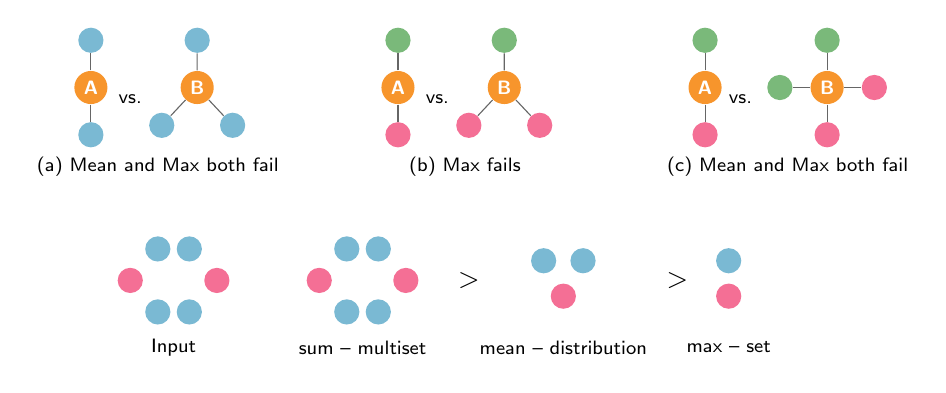
\begin{tikzpicture}
    % (a)
    \node[lec06ctr] (A) at (0,0) {A};
    \node[lec06B] (a1) at (0,0.6) {}; \node[lec06B] (a2) at (0,-0.6) {};
    \draw[black!60] (A)--(a1) (A)--(a2);
    \node[lec06lbl] at (0.5,-0.15) {vs.};
    \node[lec06ctr] (B) at (1.35,0) {B};
    \node[lec06B] (b1) at (1.35,0.6) {}; \node[lec06B] (b2) at (0.9,-0.48) {};
    \node[lec06B] (b3) at (1.8,-0.48) {};
    \draw[black!60] (B)--(b1) (B)--(b2) (B)--(b3);
    \node[lec06lbl] at (0.85,-1.0) {(a) Mean and Max both fail};
    % (b)
    \begin{scope}[shift={(3.9,0)}]
      \node[lec06ctr] (A) at (0,0) {A};
      \node[lec06G] (a1) at (0,0.6) {}; \node[lec06R] (a2) at (0,-0.6) {};
      \draw[black!60] (A)--(a1) (A)--(a2);
      \node[lec06lbl] at (0.5,-0.15) {vs.};
      \node[lec06ctr] (B) at (1.35,0) {B};
      \node[lec06G] (b1) at (1.35,0.6) {}; \node[lec06R] (b2) at (0.9,-0.48) {};
      \node[lec06R] (b3) at (1.8,-0.48) {};
      \draw[black!60] (B)--(b1) (B)--(b2) (B)--(b3);
      \node[lec06lbl] at (0.85,-1.0) {(b) Max fails};
    \end{scope}
    % (c)
    \begin{scope}[shift={(7.8,0)}]
      \node[lec06ctr] (A) at (0,0) {A};
      \node[lec06G] (a1) at (0,0.6) {}; \node[lec06R] (a2) at (0,-0.6) {};
      \draw[black!60] (A)--(a1) (A)--(a2);
      \node[lec06lbl] at (0.45,-0.15) {vs.};
      \node[lec06ctr] (B) at (1.55,0) {B};
      \node[lec06G] (b1) at (1.55,0.6) {}; \node[lec06G] (b2) at (0.95,0) {};
      \node[lec06R] (b3) at (2.15,0) {}; \node[lec06R] (b4) at (1.55,-0.6) {};
      \draw[black!60] (B)--(b1) (B)--(b2) (B)--(b3) (B)--(b4);
      \node[lec06lbl] at (1.05,-1.0) {(c) Mean and Max both fail};
    \end{scope}
    % ranking
    \begin{scope}[shift={(0.6,-2.45)}]
      \foreach \dx/\t in {0/Input, 2.4/sum -- multiset} {
        \foreach \x/\y in {0.25/0.4, 0.65/0.4, 0.25/-0.4, 0.65/-0.4}
          \node[lec06B] at (\dx+\x,\y) {};
        \foreach \x in {-0.1, 1.0} \node[lec06R] at (\dx+\x,0) {};
        \node[lec06lbl] at (\dx+0.45,-0.85) {\t};}
      \node at (4.2,0) {$>$};
      \node[lec06B] at (5.15,0.25) {}; \node[lec06B] at (5.65,0.25) {};
      \node[lec06R] at (5.4,-0.2) {};
      \node[lec06lbl] at (5.4,-0.85) {mean -- distribution};
      \node at (6.85,0) {$>$};
      \node[lec06B] at (7.5,0.25) {}; \node[lec06R] at (7.5,-0.2) {};
      \node[lec06lbl] at (7.5,-0.85) {max -- set};
    \end{scope}
  \end{tikzpicture}
  \caption{The power of pooling: failure cases of mean and max pooling (top) and
  the ranking by discriminative power (bottom) (slide~47).}
  \label{fig:lec06-pooling}
\end{figure}

\begin{table}[htbp]
  \centering\small
  \caption{Neighbor aggregation of the three models (slides~34--47).}
  \label{tab:lec06-agg}
  \renewcommand{\arraystretch}{1.2}
  \begin{tabularx}{\textwidth}{@{}l>{\raggedright\arraybackslash}p{3.6cm}l>{\raggedright\arraybackslash}Xl@{}}
    \toprule
    Model & Aggregation & Captures & Cannot distinguish & Injective?\\
    \midrule
    GCN & element-wise mean $\to$ Linear $\to$ ReLU & distribution
        & multi-sets with the same color proportion & no\\
    GraphSAGE & MLP $\to$ element-wise max & set
        & multi-sets with the same set of distinct colors & no\\
    GIN & MLP $\to$ element-wise sum $\to$ MLP & multiset
        & -- (no failure cases) & yes\\
    \bottomrule
  \end{tabularx}
\end{table}

\subsection{Full model of GIN: the WL graph kernel}\label{sec:lec06-wl}
\slides{48--53}

\begin{itemize}
  \item \textbf{So far:} the neighbor aggregation part of GIN. \textbf{Now:} the
    full model of GIN, by relating it to the \term{WL graph kernel} (traditional
    way of obtaining graph-level features) $\Rightarrow$ GIN is a ``neural
    network'' version of the WL graph kernel.
  \item Recall the \textbf{graph isomorphism} problem (slide~49 repeats slide~7,
    \cref{sec:lec06-iso}).
\end{itemize}
\begin{definition}[Color refinement algorithm in WL kernel]\label{def:lec06-wl}
  \textbf{Given:} a graph $G$ with a set of nodes $V$.
  \begin{itemize}
    \item Assign an initial color $c^{(0)}(v)$ to each node $v$.
    \item Iteratively refine node colors by
      \begin{equation}\label{eq:lec06-wl}
        c^{(k+1)}(v) = \mathrm{HASH}\Big(c^{(k)}(v),\, \big\{c^{(k)}(u)\big\}_{u\in N(v)}\Big),
      \end{equation}
      where HASH maps different inputs to different colors.
    \item After $K$ steps of color refinement, $c^{(K)}(v)$ \textbf{summarizes the
      structure of $K$-hop neighborhood}.
  \end{itemize}
\end{definition}
\begin{example}[Color refinement given two graphs]
  \begin{itemize}
    \item \textbf{Assign initial colors:} every node gets color 1
      (\cref{fig:lec06-wl}).
    \item \textbf{Aggregate neighboring colors:} (own color, neighbor colors),
      e.g.\ ``1,1111'' = color 1 with four neighbors of color 1.
    \item \textbf{Injectively HASH the aggregated colors:} HASH table
      1,1 $\to$ 2; 1,11 $\to$ 3; 1,111 $\to$ 4; 1,1111 $\to$ 5 (injective!).
    \item Process continues until a \textbf{stable coloring} is reached. Two graphs
      are considered \textbf{isomorphic} if they have the same set of colors. Here
      the stable colors are $\{7,7,8,11,11,12\}\neq\{6,7,9,10,11,13\}$.
  \end{itemize}
\end{example}

\begin{figure}[htbp]
  \centering
  \begin{tikzpicture}
    \foreach \x/\t in {0/{aggregated colors}, 3.2/{after injective HASH},
                       6.2/{stable coloring}}
      \node[lec06lbl, font=\scriptsize\sffamily\bfseries] at (\x,1.12) {\t};
    \pic (a1) at (0,0) {lec06wlL={{1,111}{1,11}{1,1111}{1,111}{1,1}{1,1}}};
    \pic (a2) at (0,-1.9) {lec06wlR={{1,11}{1,111}{1,1111}{1,111}{1,1}{1,1}}};
    \pic (b1) at (3.2,0) {lec06wlL={{4}{3}{5}{4}{2}{2}}};
    \pic (b2) at (3.2,-1.9) {lec06wlR={{3}{4}{5}{4}{2}{2}}};
    \pic (c1) at (6.2,0) {lec06wlL={{11}{8}{12}{11}{7}{7}}};
    \pic (c2) at (6.2,-1.9) {lec06wlR={{9}{11}{13}{10}{7}{6}}};
    \node at (7.65,-0.95) {\large$\neq$};
    \node[draw, thick, font=\scriptsize\sffamily, align=left, inner sep=4pt,
          anchor=west] at (8.2,-0.95)
      {\textbf{HASH table}\\[1pt] 1,1 $\to$ 2\\ 1,11 $\to$ 3\\ 1,111 $\to$ 4\\
       1,1111 $\to$ 5};
  \end{tikzpicture}
  \caption{Color refinement on two graphs (top, bottom) with all initial colors 1:
  aggregated colors, colors after the injective HASH, and the stable coloring;
  different color sets $\Rightarrow$ not isomorphic (slides~51--53).}
  \label{fig:lec06-wl}
\end{figure}

\subsection{The complete GIN model}\label{sec:lec06-complete}
\slides{54--58}

\begin{itemize}
  \item \textbf{GIN uses a neural network to model the injective HASH function}
    of \cref{eq:lec06-wl}. Specifically, we model the injective function over the
    tuple (root node features $c^{(k)}(v)$, neighboring node colors
    $\{c^{(k)}(u)\}_{u\in N(v)}$).
\end{itemize}
\begin{proposition}[Xu et al.\ ICLR 2019]\label{prop:lec06-tuple}
  Any injective function over the tuple (root node feature $c^{(k)}(v)$,
  neighboring node features $\{c^{(k)}(u)\}_{u\in N(v)}$) can be modeled as
  \begin{equation}\label{eq:lec06-gintuple}
    \mathrm{MLP}_{\Phi}\Big((1+\epsilon)\cdot\mathrm{MLP}_f\big(c^{(k)}(v)\big)
      + \sum_{u\in N(v)}\mathrm{MLP}_f\big(c^{(k)}(u)\big)\Big)
  \end{equation}
  where $\epsilon$ is a learnable scalar.
\end{proposition}
\begin{itemize}
  \item If input feature $c^{(0)}(v)$ is represented as one-hot, \textbf{direct
    summation is injective} (e.g.\ $\Phi$(yellow + blue + blue):
    $\binom{1}{0}+\binom{0}{1}+\binom{0}{1}=\binom{1}{2}$) $\Rightarrow$ we only
    need $\Phi$ to ensure the injectivity (root node features $c^{(k)}(v)$,
    neighboring node features $\{c^{(k)}(u)\}_{u\in N(v)}$):
\end{itemize}
\begin{equation}\label{eq:lec06-ginconv}
  \mathrm{GINConv}\Big(c^{(k)}(v), \{c^{(k)}(u)\}_{u\in N(v)}\Big)
  = \mathrm{MLP}_{\Phi}\Big((1+\epsilon)\cdot c^{(k)}(v) + \sum_{u\in N(v)} c^{(k)}(u)\Big)
\end{equation}
\begin{itemize}
  \item This $\mathrm{MLP}_{\Phi}$ can provide ``one-hot'' input feature for the
    next layer.
  \item \textbf{GIN's node embedding updates.} Given a graph $G$ with a set of
    nodes $V$: assign an \textbf{initial vector} $c^{(0)}(v)$ to each node $v$;
    iteratively update node vectors by
\end{itemize}
\begin{equation}\label{eq:lec06-ginupdate}
  c^{(k+1)}(v) = \mathrm{GINConv}
    \Big(\big\{c^{(k)}(v), \{c^{(k)}(u)\}_{u\in N(v)}\big\}\Big),
\end{equation}
\begin{itemize}
  \item[] GINConv = \textbf{differentiable color HASH function}; it maps
    different inputs to different embeddings. After $K$ steps of GIN iterations,
    $c^{(K)}(v)$ \textbf{summarizes the structure of $K$-hop neighborhood}.
  \item GIN can be understood as a \textbf{differentiable neural version of the WL
    graph kernel} (\cref{tab:lec06-wlgin}).
  \item \textbf{Advantages of GIN over the WL graph kernel:} node embeddings are
    \textbf{low-dimensional}; hence, they can capture the fine-grained similarity
    of different nodes. Parameters of the update function can be \textbf{learned
    for the downstream tasks}.
\end{itemize}

\begin{table}[htbp]
  \centering\small
  \caption{GIN as the neural version of the WL graph kernel (slide~58).}
  \label{tab:lec06-wlgin}
  \begin{tabular}{@{}lll@{}}
    \toprule
    & Update target & Update function\\
    \midrule
    WL graph kernel & node colors (one-hot) & HASH\\
    GIN & node embeddings (low-dim vectors) & GINConv\\
    \bottomrule
  \end{tabular}
\end{table}

\subsection{Expressive power of GIN and its limits}\label{sec:lec06-limits}
\slides{59--64}

\begin{itemize}
  \item Because of the relation between GIN and the WL graph kernel, \textbf{their
    expressive power is exactly the same}: if two graphs can be distinguished by
    GIN, they can be also distinguished by the WL kernel, and vice versa.
  \item \textbf{How powerful is this?} WL kernel has been both theoretically and
    empirically shown to distinguish most of the real-world graphs [Cai et al.\
    1992] $\Rightarrow$ GIN is also powerful enough to \textbf{distinguish most of
    the real graphs}!
  \item \textbf{Some bad news:}
    \begin{itemize}
      \item The WL kernel cannot distinguish between some basic graph structures,
        e.g.\ two 5-cycles joined by an edge vs.\ two 6-cycles sharing an edge
        (\cref{fig:lec06-limits}a).
      \item The WL kernel cannot count important sub-structures, e.g.\
        \textbf{cycles} and \textbf{cliques}.
    \end{itemize}
  \item \textbf{Why do we care about cycles?} The \textbf{bonds between different
    atoms} in chemical compounds form \textbf{cycles}. The hexagon is the
    \textbf{most common polygon} in organic compounds $\Rightarrow$ yields stable
    materials (e.g.\ doxorubicin, camptothecin, etoposide).
  \item \textbf{Why cliques and quasi-cliques?}
    \begin{itemize}
      \item Fraudster detection in e-commerce networks [Hooi et al.\ 2016]:
        users $\times$ objects adjacency; fraudsters form a dense block with the
        customers' objects, plus camouflage (biased) edges to honest objects.
      \item Detection of protein complexes in PPI networks [Vlaic et al.\ 2017].
      \item Graph compression [Dhulipala et al.\ 2017] (dense blocks of the
        adjacency matrix).
    \end{itemize}
  \item \textbf{Improving GNNs' power -- can the expressive power of GNNs be
    improved?}
    \begin{itemize}
      \item There are basic graph structures that the existing GNN framework cannot
        distinguish, such as difference in cycles: $v_1$ in a triangle (A) and
        $v_2$ in a square (B) have the \textbf{same computational graphs}
        (\cref{fig:lec06-limits}b).
      \item GNNs' expressive power \textbf{can be improved} to resolve the above
        problem [You et al.\ AAAI 2021, Li et al.\ NeurIPS 2020, Kanatsoulis et al.\
        ICLR 2024].
    \end{itemize}
\end{itemize}

\begin{figure}[htbp]
  \centering
  \begin{subfigure}[b]{0.52\textwidth}
    \centering
    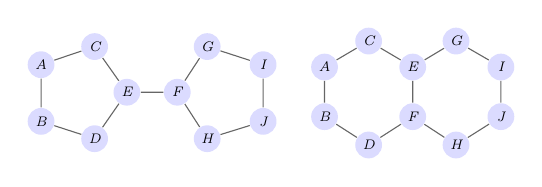
\begin{tikzpicture}
      \foreach \n/\x/\y in {A/0/0.35, C/0.68/0.58, E/1.09/0, D/0.68/-0.59,
          B/0/-0.37, F/1.73/0, G/2.11/0.58, I/2.82/0.35, J/2.82/-0.37, H/2.11/-0.59}
        \node[lec06s] (p\n) at (\x,\y) {\n};
      \draw[black!60] (pA)--(pC)--(pE)--(pD)--(pB)--(pA) (pE)--(pF)
        (pF)--(pG)--(pI)--(pJ)--(pH)--(pF);
      \foreach \n/\x/\y in {A/3.6/0.32, C/4.16/0.65, E/4.72/0.32, F/4.72/-0.31,
          D/4.16/-0.67, B/3.6/-0.31, G/5.27/0.65, I/5.84/0.32, J/5.84/-0.31, H/5.27/-0.67}
        \node[lec06s] (q\n) at (\x,\y) {\n};
      \draw[black!60] (qA)--(qC)--(qE)--(qF)--(qD)--(qB)--(qA)
        (qE)--(qG)--(qI)--(qJ)--(qH)--(qF);
    \end{tikzpicture}
    \caption{Two graphs the WL kernel cannot distinguish (slide~60).}
  \end{subfigure}\hfill
  \begin{subfigure}[b]{0.44\textwidth}
    \centering
    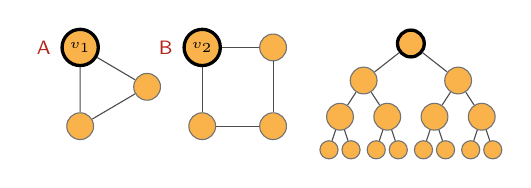
\begin{tikzpicture}[lf/.style={lec06n, minimum size=2.3mm}]
      \node[lec06rt, minimum size=4.6mm, label={[text=BrickRed, font=\scriptsize\sffamily]left:A}] (t1) at (0,0.5) {\tiny$v_1$};
      \node[lec06n] (t2) at (0.85,0) {}; \node[lec06n] (t3) at (0,-0.5) {};
      \draw[black!70] (t1)--(t2)--(t3)--(t1);
      \node[lec06rt, minimum size=4.6mm, label={[text=BrickRed, font=\scriptsize\sffamily]left:B}] (s1) at (1.55,0.5) {\tiny$v_2$};
      \node[lec06n] (s2) at (2.45,0.5) {}; \node[lec06n] (s3) at (2.45,-0.5) {};
      \node[lec06n] (s4) at (1.55,-0.5) {};
      \draw[black!70] (s1)--(s2)--(s3)--(s4)--(s1);
      % computational graph (same for v1 and v2)
      \node[lec06rt] (r) at (4.2,0.55) {};
      \foreach \i/\x in {1/3.6, 2/4.8} {
        \node[lec06n] (c\i) at (\x,0.08) {}; \draw[black!70] (r)--(c\i);
        \foreach \j/\dx in {1/-0.3, 2/0.3} {
          \node[lec06n] (d\i\j) at (\x+\dx,-0.38) {}; \draw[black!70] (c\i)--(d\i\j);
          \foreach \k/\ddx in {1/-0.14, 2/0.14}
            {\node[lf] (e) at (\x+\dx+\ddx,-0.8) {}; \draw[black!70] (d\i\j)--(e);}}}
    \end{tikzpicture}
    \caption{Triangle vs.\ square: identical computational graphs for $v_1$ and
    $v_2$ (slide~63).}
  \end{subfigure}
  \caption{Limits of WL / message-passing GNNs (slides~60, 63).}
  \label{fig:lec06-limits}
\end{figure}

\paragraph{Summary of the lecture} (slide~64). We design a neural network that
can model an \textbf{injective multi-set function} and use it for the neighbor
aggregation function $\Rightarrow$ \textbf{GIN -- the most expressive GNN model}.
The key is to use \textbf{element-wise sum pooling}, instead of mean-/max-pooling.
GIN is closely related to the WL graph kernel; both GIN and WL graph kernel can
distinguish most of the real graphs!

% ---------------------------------------------------------------------
\bigskip\phantomsection
\addcontentsline{toc}{section}{Lecture 6 at a glance}
\begin{summarybox}[Lecture 6 at a glance]
  \begin{itemize}
    \item \textbf{Expressive power} = ability to distinguish graph structures;
      classical test: graph isomorphism.
    \item \textbf{Computational graph = rooted subtree}; GNN sees features, not
      IDs $\Rightarrow$ identical subtrees (nodes 1, 2) $\Rightarrow$ identical
      embeddings. Most expressive GNN $\Leftrightarrow$ \textbf{injective neighbor
      aggregation at every step}.
    \item Aggregation = function over a \textbf{multi-set}. GCN (mean) fails on
      equal color proportions, GraphSAGE (max) on equal sets of distinct colors.
      Ranking: sum (multiset) $>$ mean (distribution) $>$ max (set).
    \item Injective multi-set function $=\Phi(\sum_{x\in S}f(x))$ + universal
      approximation $\Rightarrow$ \textbf{GIN:}
      $\mathrm{MLP}_{\Phi}(\sum_{x\in S}\mathrm{MLP}_f(x))$, injective.
    \item \textbf{WL:} $c^{(k+1)}(v)=\mathrm{HASH}(c^{(k)}(v),
      \{c^{(k)}(u)\}_{u\in N(v)})$; \textbf{GINConv}
      $=\mathrm{MLP}_{\Phi}((1+\epsilon)\cdot c^{(k)}(v)+\sum_{u\in N(v)}c^{(k)}(u))$
      is its differentiable version; GIN $\equiv$ WL in power.
    \item \textbf{Limits:} cannot count cycles or cliques (triangle vs.\ square);
      expressive power can be improved.
  \end{itemize}
\end{summarybox}
